
\begin{concept}[15cm]
\textit{Nội dung chương này sẽ tập trung giới thiệu tổng quan về BE-PUM, điểm mạnh của công vụ này và so sánh với công cụ khác, những đòi hỏi trong quá trình hiện thực công cụ và yếu tố quyết  định để cho ra đề tài này; dẫn nhập về hợp ngữ assembly, dẫn nhập về Windows API, các thành phần sẽ được áp dụng để phát triển cho BE-PUM; nêu ra mục tiêu của đề tài và giới hạn trong phạm vi luận văn tốt nghiệp.}
\end{concept}

\section{Giới thiệu về BE-PUM}
	\subsection{BE-PUM là gì}

BE-PUM tên đầy đủ là Binary Emulation for Pushdown Model generation, là một công cụ dùng để phân tích động mã nhị phân của một chương trình bất kỳ chạy trên kiến trúc X86 của hệ điều hành Microsoft Windows nền tảng 32-bit. Sau khi phân tích, BE-PUM sẽ sinh ra hợp ngữ – mã assembly và đồ thị luồng điều khiển (control flow graph – CFG) của chương trình đầu vào.\\

BE-PUM được xây dựng chính trên mã nguồn của JakStab, nhưng không hạn hẹp ở việc chỉ phân tích tĩnh, BE-PUM có thể phân tích động và chỉ ra lại mỗi dòng lệnh của mã assembly môi trường làm việc của nó là như thế nào. Việc này sẽ giải quyết được những hạn chế mà phương pháp phân tích tĩnh không thể xử lý được.

	\subsection{Mục tiêu hướng đến của BE-PUM}

Với cuộc sống ngày càng hiện đại của con người, sự phổ biến và tầm quan trọng của máy tính ngày càng nâng cao. Các công việc quan trọng nay hầu hết đều có thể được quản lý và xử lý bởi các phần mềm máy tính, từ các hệ thống quản lý nhân công hay các quy trình tài chính, ngân hàng. Sự lệ thuộc nhiều vào máy tính đó đã kéo theo cho sự ra đời của hàng loạt những phần mềm độc hại, với các mục đích xấu, đôi lúc chỉ là để mua vui hay nghiêm trọng hơn là tư lợi cho bản thân người viết ra chúng. \\

Bằng việc phân tích mã nhị phân, BE-PUM đang được phát triển để tập trung vào việc phân tích những phần mềm bị nghi ngờ, sau đó dựa vào hành vi sẽ phát hiện được những kỹ thuật tấn công, và cuối cùng là xác định xem đây có thực là phần mềm gây hại đến máy tính (malware - malicious software) hay không?

	\subsection{Các hướng tiếp cận}

Với một công cụ phân tích tập trung vào phần mềm độc hại, ta có một số hướng tiếp cận như sau:
		\subsubsection{Phát hiện dựa trên dấu hiệu}
Phát hiện dựa trên dấu hiệu (signature detection) là một hướng tiếp cận theo kiểu công nghiệp, nó được dùng trong đại đa số các phần mềm phát hiện malware vì đặc tính là nhanh chóng xác định một malware; nhưng đi kèm là hạn chế chỉ phát hiện được trong giới hạn một lượng dấu hiệu đã nạp sẵn.\\

Khi một chương trình phát hiện malware thông thường thực hiện việc quét tìm mối nguy hiểm, chúng sẽ kiểm tra nội dung của từng tập tin, so trùng nội dung đó với bộ từ điển các dấu hiện đã có sẵn và nhận biết. Việc này sẽ đòi hỏi bộ từ điển kia được cập nhật liên tục từ nhà phát hành, nhưng việc cập nhật đó cũng chỉ có giới hạn, trong khi các malware được gia tăng qua từng ngày. Việc một malware sinh ra biến thể nhỏ có thể khiến cho một dấu hiệu nhận dạng trước đó không hoạt động chính xác nữa.

		\subsubsection{Phát hiện dựa vào giả lập}
Dựa vào bộ giả lập (emulation) là một cách tiếp cận với việc xây dựng và thực thi tập tin malware trong một môi trường sandbox. Môi trường sandbox là môi trường ảo hóa được dựng lên với các tính năng tương tự như một hệ thống thật, nhưng cách ly và bị hạn chế không thể tạo ra một thay đổi lâu dài. Điều này có nghĩa là tất cả những gì xảy ra trong sandbox sẽ chỉ ở trong sandbox.\\

Nhưng một malware tinh vi có thể phát hiện được rằng chúng đang chạy trong sandbox và ta sẽ không thu được kết quả gì. Cộng thêm với việc xây dựng một môi trường sandbox đòi hỏi bỏ ra rất nhiều công sức, và hành vi của một malware sẽ có thể bị khác nhau (do thực thi thật) ở nhiều thời điểm; do đó phương pháp này không được nhắm tới.

		\subsubsection{Phát hiện dựa vào sinh mô hình}

Sinh mô hình (model generation) là một cách tiếp cận hình thức với việc mọi câu lệnh được mô hình hóa và biểu diễn bằng mô hình. Sau khi xử lý một chuỗi các mô hình qua các câu lệnh có trong tập tin, ta sẽ có được đồ thị luồng điều khiển và giải quyết bài toán trên đó bằng phương pháp kiểm tra mô hình (model checking).

	\subsection{Đồ thị luồng điều khiển}

\textit{Đồ thị luồng điều khiển (control flow graph - CFG)} trong khoa học máy tính là một phép biểu diễn của tất cả các đường có thể được duyệt qua trong quá trình thực thi của một chương trình. \cite{cfg-def}\\

Trong BE-PUM, một địa chỉ trong chương trình được ánh xạ tương ứng với 1 nút (node) trong đồ thị. BE-PUM sẽ xử lý theo luồng thực thi của chương trình và sinh ra từng nút một tương ứng. Trong quá trình xử lý, BE-PUM sẽ quyết định được điểm kế tiếp cần đi đến trong lúc duyệt nhánh. Tất cả việc đó được thực hiện thông qua giải thuật \textit{on-the-fly model generation}.\\

\textit{On-the-fly model generation} là giải thuật chính trong hệ thống BE-PUM. Quá trình thực thi của tập tin mã nhị phân là một chuỗi thực thi động, bắt đầu từ một giá trị trong ở phân vùng mã (code section) của bộ nhớ, giá trị địa chỉ này được chỉ rõ bởi giá trị thanh ghi EIP. BE-PUM sẽ đặt khởi điểm từ đây, và lần dò theo từng câu lệnh hợp ngữ, tìm điểm kế tiếp sẽ được thực thi. Cứ như vậy, BE-PUM sẽ đi qua hết các nhánh có khả năng thực thi của chương trình và cho ra một đồ thị luồng điều khiển đầy đủ.

	\subsection{Ví dụ đơn giản về sinh ra đồ thị CFG bằng BE-PUM}

Để hiểu rõ hơn về công việc của BE-PUM, ta cùng xem qua một ví dụ minh họa nhỏ về việc sinh ra đồ thị luồng điều khiển (Hình \ref{fig:imgexcfg}) với một đoạn mã hợp ngữ ở Bảng \ref{table:tblexcfg}.

\begin{longtable}{ | m{3cm} | m{5cm} | }
	\hline
Địa chỉ câu lệnh & Nội dung câu lệnh\\
	\hline
	\hline
0x00401000 & cmp eax, 0 \\
	\hline
0x00401003	& je 0x0040100d \\
	\hline
0x00401005 & mov eax, 0x00401001 \\
	\hline
0x0040100a & jmp 0x00401015 \\
	\hline
0x0040100c & ret \\
	\hline
0x0040100d & mov eax, 0x00401018 \\
	\hline
0x00401012 & add eax, 10 \\
	\hline
0x00401015 & sub eax, 4 \\
	\hline
0x00401015 & ret \\
	\hline

\caption{Nội dung của một tập tin nhị phân dưới dạng hợp ngữ (1)}
\label{table:tblexcfg}
\end{longtable}

\begin{figure}[H]
\centering
\begin{tikzpicture}
[->,>=stealth',shorten >=1pt,auto,node distance=2cm,thick,main node/.style={circle,draw}]

\node[main node] (00) {00};
\node[main node] (03) [below of=00] {03};
\node[main node] (0A) [below of=03] {0A};
\node[main node] (05) [right of=0A] {05};
\node[main node] (0D) [left of=0A] {0D};
\node[main node] (12) [below of=0D] {12};
\node[main node] (15) [below of=0A] {15};
\node[main node] (18) [right of=15] {18};


\path[every node/.style={font=\sffamily\small}]
    	(00) edge node [left] {} (03)
    	(03) edge [bend left] node [left] {} (05)
        	       edge [bend right] node[left] {} (0D)
    	(05) edge node [left] {} (0A)
    	(0D) edge node [left] {} (12)
    	(0A) edge node [left] {} (15)
	(15) edge node [left] {} (18)
	(12)edge node[left] {} (15)
	;
\end{tikzpicture}
\caption{Đồ thị luồng điều khiển được sinh ra từ tập tin ở Bảng \ref {table:tblexcfg}} 
\label{fig:imgexcfg}
\end{figure}

	\subsection{Những đòi hỏi trong quá trình hiện thực}

Đối với những tập tin nhị phân đơn giản, ta có thể dễ dàng quyết định được nút kế tiếp. Nhưng với những malware tinh vi, chúng sẽ có cách để ta không dễ dàng hiểu được ý định chúng sẽ làm gì, ra sao. Phương thức trên được gọi là làm rối mã (obfuscation). Một trong những cách điển hình có thể kể đến là nhảy gián tiếp (indirect jump -- thực hiện lệnh nhảy đến một giá trị không phải là hằng số như giá trị thanh ghi, giá trị ô nhớ...) và tự thay đổi mã (self-modification code -- trong quá trình thực thi sẽ tự ý thay đổi nội dung mã thực thi của chính mình).\\

Và BE-PUM đã được dựng lên để có thể chống lại việc làm rối mã này. Đó là điểm mạnh và là ưu thế vượt trội của BE-PUM so với các công cụ phân tích tĩnh mã thực thi khác như Jackstab, IDA Pro, Capstone, Unicorn, METASM, HOOPER bằng việc áp dụng phương pháp \textit{dynamic symbolic execution}.\\

\textit{Dynamic symbolic execution} là một phương pháp nhằm tính toán các giá trị thanh ghi và bộ nhớ ở một vị trí cụ thể, khi chúng ta không thể biết được điểm thực thi kế tiếp của chương trình là gì. Nhờ đó ta có thể giải quyết được các cách thức làm rối mã như nhảy gián tiếp, tự thay đổi mã như đã nói ở trên.\\

Để có thể tính toán được các giá trị thanh ghi cũng như bộ nhớ, ta cần xây dựng một hệ thống mô phỏng các câu lệnh mà một tập tin nhị phân thực hiện được. Các câu lệnh đó bao gồm 2 phần chính đó là \textit{hợp ngữ} và \textit{Windows API}.\\

\textbf{\textit{Đây là lý do chính hình thành nên đề tài luận văn này.}}

	\subsection{Ví dụ so sánh giữa BE-PUM và IDA Pro}

Đây là một ví du so sánh giữa BE-PUM và công cụ dịch ngược điển hình, rất nổi tiếng khác đó là IDA Pro, để cho thấy rõ được điểm mạnh và sự khác biệt của BE-PUM so với các công cụ khác.

\begin{longtable}{ | m{3cm} | m{5cm} | }
	\hline
Địa chỉ câu lệnh & Nội dung câu lệnh\\
	\hline
	\hline
0x00401000 & cmp eax, 0 \\
	\hline
0x00401003	& jne 0x00401015 \\
	\hline
0x00401005 & call 0x00401011 \\

	\hline
0x0040100a & add eax, 09h \\
	\hline
0x0040100d & inc eax \\
	\hline
0x0040100e & inc eax \\
	\hline
0x0040100f & jmp eax \\

	\hline
0x00401015 & push 0 \\
	\hline
0x00401017 & call  0x0040101c\\
	\hline
0x0040101c & jmp ExitProcess\\

	\hline
0x00401011 & mov eax, ss:[esp] \\
	\hline
0x00401014 & ret \\
	\hline

\caption{Nội dung của một tập tin nhị phân dưới dạng hợp ngữ (2)}
\label{table:tblAsmEx2}
\end{longtable}


\newpage

Nhìn vào đoạn mã ở Bảng \ref{table:tblAsmEx2}, ta nhận thấy tại địa chỉ \textit{0x0040100f} có thực hiện câu lệnh nhảy gián tiếp. Đối với các công cụ chạy trên mô hình phân tích tĩnh thì khi phân tích đến vị trí này, công cụ đó sẽ không thể tìm được điểm cần nhảy đến nữa và sẽ dừng việc phân tích ở đây lại. Ta có thể dễ dàng thấy được điều đó qua Hình \ref{fig:ModelReal} (b) ngay sau đây.\\

Nhưng đối với BE-PUM, một công cụ hỗ trợ cả phân tích tĩnh và phân tích động, thì tại điểm này, BE-PUM có thể tính toán được giá trị cần nhảy đến và dễ dàng tìm được điểm đích cần xử lý tiếp theo. Hình \ref{fig:ModelReal} (a) đã miêu tả rõ ràng được điều đó qua việc nút \textit{0x0040100f} đã liên thông đến nút cần xử lý là \textit{0x00401015}.

\newpage

\begin{figure}[H]
\centering
\begin{tabular}[c]{cc}
	\subfloat[BE-PUM]
	{
		\label{fig:BEPUMReal}
		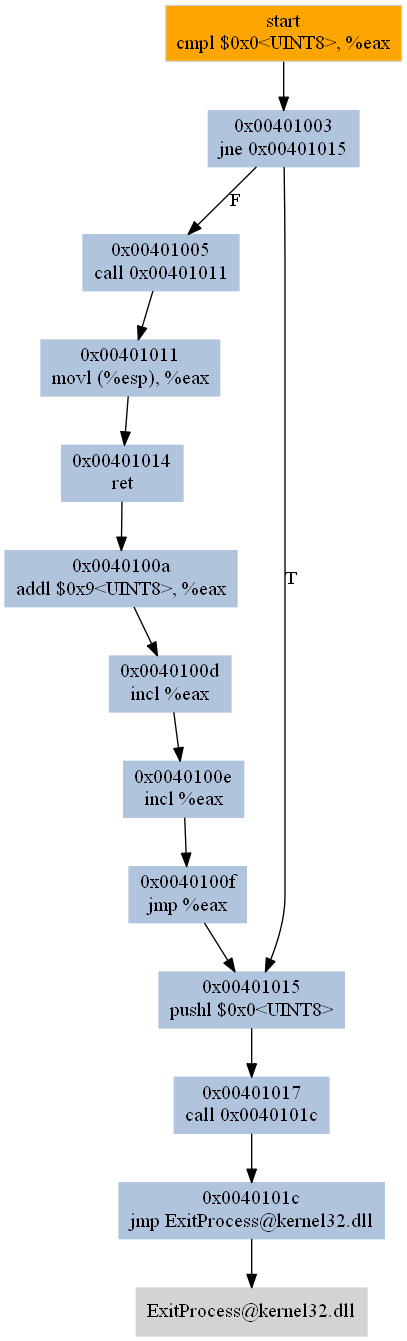
\includegraphics[width=0.4\textwidth]{bepum_sample}
    }
    &
	\subfloat[IDA Pro]
	{
		\label{fig:IDAReal}
        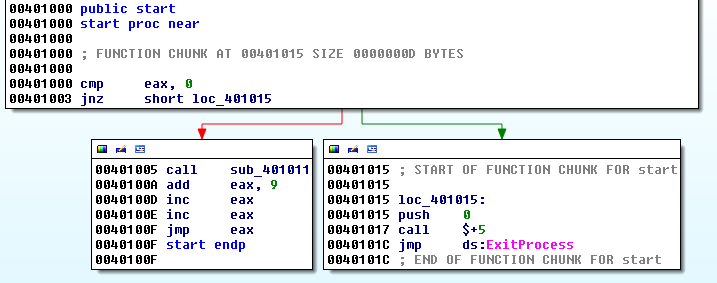
\includegraphics[width=0.6\textwidth]{ida_sample}
	}
\end{tabular}
\caption{Mô hình của BE-PUM và IDA Pro được sinh ra từ đoạn mã ở Bảng \ref {table:tblAsmEx2}}
\label{fig:ModelReal}
\end{figure}

\section{Tổng quan về hợp ngữ}
Ngôn ngữ assembly (hay hợp ngữ) là ngôn ngữ cấp thấp được biên dịch để thực thi một chương trình nào đó. Ngôn ngữ assembly có tính gợi nhớ, mỗi câu lệnh thực thi một chức năng, hay nhiệm vụ riêng biệt tương ứng với một lệnh yêu cầu máy thực thi. \\

Các chương trình sau khi biên dịch ra thành nhiều dạng file khác nhau để thực thi. Mỗi chương trình được biên dịch thành ngôn ngữ assembly trước khi biên dịch qua ngôn ngữ máy để máy hiểu và thực thi câu lệnh. Khi biên dịch qua mã assembly, đọc đoạn mã assembly để phân tích xem chương trình này có phải là virus máy tính không, có những hành vi bất thường từ đó xem xét đưa ra kết quả chương trình này có an toàn với máy tính.

\section {Tổng quan về Windows API}

Với tên gọi đầy đủ là Microsoft Windows application programming interface, đôi lúc được gọi một cách ngắn gọn là WinAPI, đây là một bộ giao diện lập trình ứng dụng (API) lõi có sẵn trong hệ điều hành Microsoft Windows (hay thường được gọi ngắn gọn là Windows).\\

Windows API là tên gọi chung của những dự án được triển khai cho những nền tảng khác nhau được áp dụng trong hệ điều hành Windows; mà thông thường chúng có những tên gọi riêng. Một số tên gọi và mô tả cho những phiên bản xin được trình bày trong Bảng \ref{table:tblwapiver}.\\

\newpage

\begin{longtable}{ | m{3cm} | m{11cm} | }
	\hline
Tên của phiên bản Windows API & Mô tả \\
	\hline
	\hline
Win16 & Đây là tên gọi bộ API đầu tiên có trong phiên bản Microsoft Windows 16-bit. Thuở ban đầu bộ API này có tên gọi là “Windows API”, nhưng sau khi phiên bản kế tiếp là Win32 ra đời, nó được đổi tên thành Win16. Lúc này các chức năng của Win16 API chủ yếu nằm trong các tập tin lõi của hệ điều hành như kernel.exe (hoặc krnl286.exe hoặc krnl386.exe), user.exe và gdi.exe. Dù rằng phần mở rộng là exe, nhưng thực tế đây là các thư viện liên kết động. \\
	\hline
Win32 & Đây là tên gọi cho bộ Windows API trong phiên bản Windows 32-bit, được giới thiệu lần đầu cùng hệ điều hành Windows NT. Các chức năng của Win32 API cũng bao gồm cả những chức năng của Win16 API, nhưng khác với phiên bản trước, chúng được đóng gói trong các tập tin DLL; trong đó có thể kể đến những tập tin DLL cốt lõi của Win32 API như: kernel32.dll, user32.dll, và gdi32.dll. \\
	\hline
Win64 & Đây là một biến thể sau đó của bộ API được hiện thực trong nền tảng Windows 64-bit. Cả chương trình 32-bit hoặc 64-bit đều có thể được biên dịch với cùng một mã nền duy nhất, dù rằng một số API trong Win32 đã được thay thế và loại bỏ. Tất cả con trỏ trong phiên bản này mặc định là 64-bit, do đó cần kiểm tra khả năng tương thích trong mã nguồn và viết lại nếu cần thiết. \\
	\hline

\caption[Một số phiên bản chính của Windows API]{Một số phiên bản chính của Windows API}
\label{table:tblwapiver}
\end{longtable}

\section{Mục tiêu đề tài}

Trong phạm vi của đề tài luận tốt nghiệp, mục tiêu nhắm tới là phát triển hệ thống xử lý các câu lệnh hợp ngữ và Windows API cho BE-PUM.\\

Với số lượng các API rất lớn hiện có trong hệ điều hành Windows, hiện tại đề tài đang tập trung vào xử lý các API ở phiên bản Win32 API, do hầu hết các phần mềm độc hại mà BE-PUM hướng tới vẫn đang dùng bộ API này; với sự ưu tiên từng bước xây dựng cho các API được dùng phổ biến trước.\\

Bên cạnh việc nhận thông tin đầu vào từ vùng nhớ đã được xây dựng của BE-PUM và trả về kết quả sau khi gọi API vào đúng địa chỉ cần thiết, điều quan trọng là phải đảm bảo không gây ngắt quãng cũng như tránh nguy hại hệ thống đang chạy. Và như vậy với những tương tác vật lý từ lời gọi API (bộ lưu trữ máy tính, cơ sở dữ liệu registry…) hay tương tác người dùng (API tạo cửa sổ message box, lệnh cho một thread “ngủ đông” trong một khoảng thời gian,…) cần được kiểm soát để không làm ảnh hưởng tới kết quả thực thi của BE-PUM.\\

\textit{Lưu ý: do nội dung đề tài tập trung vào xử lý cho Win32 API, nên kể từ đây, khi báo cáo nhắc đến Windows API tức là nói đến Win32 API.}\\

Việc hiện thực các câu lệnh hợp ngữ góp phần phân tích một số loại malware đang nghiên cứu. Dựa trên một số bộ malware hiện nay và những câu lệnh phổ biến thường gặp, BE-PUM sẽ hỗ trợ tốt công việc phân tích đúng môi trường làm việc của từng câu lệnh từ đó xác định chính xác và phân tính đúng các kỹ thuật mà malware đang tiến hành.

\newpage
\section{Giới hạn đề tài}

Trong phạm vi của đề tài luận văn tốt nghiệp, mục tiêu nhắm tới là hiện thực các câu lệnh hợp ngữ và Windows API với số lượng đạt mức như sau:

\begin{itemize}
  \item Số lượng câu lệnh hợp ngữ được hỗ trợ đạt khoảng 250 câu lệnh.
  \item Số lượng câu lệnh Windows API được hỗ trợ đạt khoảng 400 câu lệnh.
\end{itemize}

\section{Cấu trúc của báo cáo}

Bài báo cáo này bao gồm những đề mục sau đây:

\begin{description}
  	\item[Chương 1] \hfill \\
	Giới thiệu tổng quan về BE-PUM, điểm mạnh của công vụ này và so sánh với công cụ khác, những đòi hỏi trong quá trình hiện thực công cụ và yếu tố quyết  định để cho ra đề tài này; dẫn nhập về hợp ngữ assembly, dẫn nhập về Windows API, các thành phần sẽ được áp dụng để phát triển cho BE-PUM; nêu ra mục tiêu của đề tài và giới hạn trong phạm vi luận văn tốt nghiệp. \\
 	\item[Chương 2] \hfill \\
	Đem đến những cái nhìn về những vấn đề đã và đang được lưu tâm khi thực hiện đề tài này; sự phổ biến của Windows API trong những phần mềm độc hại để thấy sự cần thiết của việc xây dựng một bộ xử lý Windows API cho BE-PUM; những khó khăn khi thực hiện điều đó và giải pháp cho vấn đề. Đông thời phân tích vấn đề đặt ra là hiện thực các câu lệnh trong hợp ngữ assembly, giải thích tại sao sử dụng ngôn ngữ assembly để tiến hành phân tích chương trình.\\
	\item[Chương 3] \hfill \\
	Trình bày những kiến thức cần thiết cho quá trình thực hiện đề tài; từ những kiến thức phải nắm được về hệ thống BE-PUM do đây là một đề tài làm việc dựa trên đó; và mỗi khi làm việc với một thư viện bất kỳ, đòi hỏi ta phải tìm hiểu cách thức làm việc với thư viện đó và cả những kiến thức cần thiết do bộ thư viện ấy yêu cầu. Đồng thời cũng trình bày các kiến thức cơ bản về hợp ngữ assembly, từ đó có cái nhìn tổng quan về assembly để tiến hành xây dựng chương trình BE-PUM. \\
	\item[Chương 4] \hfill \\
	Mỗi chương trình bất kỳ đều cần một thiết kế tốt để giúp cho việc xây dựng dễ dàng và quy chuẩn hơn. Mục này sẽ trình bày cách mà bộ xử lý Windows API đã được hiện thực để tương tai sau này có thể dễ dàng sửa chữa, bảo trì và bổ sung thêm vào kiến trúc đó. Để hiểu rõ cấu chương trình mô phỏng câu lệnh assembly, sơ đồ class trình bày trong chương này thể hiện được mối quan hệ giữa các class, cấu trúc của chương trình BE-PUM được phát triển dựa trên dự án JakStab, giới thiệu các class quan trọng của chương trình BE-PUM.\\
	\item[Chương 5] \hfill \\
	 Trình bày và phân tích, so sánh với các công cụ khác về kết quả mà đề tài đã đạt được sau khi tiến hành thực hiện công việc, kết quả tổng thể mà bộ xử lý đã được đóng góp để hỗ trợ cho hệ thống BE-PUM.\\
	\item[Chương 6] \hfill \\
	 Sau khi có được những kết quả ở thời điểm hiện tại của quá trình thực hiện đề tài, chương cuối này sẽ trình bày về những phương hướng cần tiếp tục phát triển trong tương lai đối với đề tài hiện tại.\\
	\item[Phụ Lục] \hfill \\
	 Liệt kê về những tài liệu và nguồn tham khảo có liên quan đến đề tài này.\\
\end{description}
